

\section{Introduction}



In 2017, Oleson et al. introduced a method for detecting time-specific differences in the trajectory of outcomes between experimental groups \cite{oleson2017detecting}. Particularly in the case of a densely sampled time series, the construction of evaluating differences at each point in time results in a series of highly correlated test statistics expanding the family-wise error rate, accommodated with an adjustment to the nominal alpha based on this autocorrelation. This was followed up with in 2018 with the introduction of the \xt{bdots} package to CRAN \cite{seedorff2018bdots}. Here, we introduce the second version of \texttt{bdots}, an update to the package that broadly expands the capabilities of the original. 

This manuscript is not intended to serve as a complete guide for using the \xt{bdots} package. Instead, the purpose is to showcase major changes and improvements, with those seeking a more comprehensive treatment directed to the package vignettes. Rather than taking a ``compare and contrast" approach, we will first enumerate the major changes, followed by a general demonstration of the package use:

\begin{singlespace}
\begin{enumerate}
\item Major changes to underlying methodology with implications for prior users of the package
\item Simplified user interface
\item Introduction of user defined curves
\item Permit fitting for arbitrary number of groups
\item Automatic detection of paired tests based on subject identifier
\item Allows for non-homogeneous sampling of data across subjects and groups
\item Introduce formula syntax for bootstrapping difference function
\item Interactive refitting process
\end{enumerate}
\end{singlespace}


We start by clearly delineating the type of problem that \xt{bdots} has been created to solve.

\paragraph{Bootstrapped differences in time series}

A typical problem in the analysis of differences of time series, and the kind that \xt{bdots} is intended to solve, involves that of two or more experimental groups containing subjects whose responses are measured over time. This may include the growth of tumors in  mice or the change in the proportion of fixations over time in the context of the VWP. In either case, we assume that each of the subjects $i = 1, \dots, n$ in the groups being considered has observed data of the following form:

\begin{equation}\label{eq:mean_structure}
y_{it} = f(t | \theta_i) + \epsilon_{it} 
\end{equation}


where $f$ represents a functional mean structure while the error structure of $\epsilon_{it}$ is open to being either IID or possess an AR(1) structure. At present, \xt{bdots} requires that each of the subjects being compared have the same parametric function $f$, though is not strictly necessary at the theoretical level and future directions of the package include accommodating non-parametric functions. While each of the subjects are required to be of the same parametric form $f(\cdot | \theta)$, each differs in their instance of their own subject-specific parameters, $\theta_i$.

An explicit assumption of the current iteration of \xt{bdots} is that each subject $i$s' parameters within a group $g = 1, \dots, G$ is drawn from a group level distribution

\begin{equation}\label{eq:group_dist}
\theta_i \sim N(\mu_g, V_g).
\end{equation}
Bootstrapping parameters to estimate this distribution and evaluating the function $f$ at these values gives us an estimate of the distribution of functions. As these function are \textit{in time}, this in turn gives a representation of the temporal changes in group characteristics. It is precisely the identification of if and when these temporal changes differ between groups that \xt{bdots} seeks to perform.


\paragraph{Homogeneous Means Assumption}

The assumption presented in Equation~\ref{eq:group_dist} differs from the original iteration of \xt{bdots} in a critical way. In \cite{oleson2017detecting}, there was no assumption of variability between subject parameters, leading to the implicit assumption that $\theta_i = \theta_j$ for all subjects $i, j$ within an experimental group. The most relevant consequence of the homogeneous means assumption is that only within-subject variability is estimated, inflating the type I error when this assumption did not hold. We investigate this in detail in Chapter 3. For now, we will give a methodological overview of the process used by \xt{bdots} along with a presentation of an updated bootstrapping process and the introduction of a permutation test.




\section{Methodology and Overview} 

A standard analysis using \xt{bdots} consists of two steps: fitting the observed data to a specified parametric function, $f(\cdot|\theta)$, and then using the observed variability to construct estimates of the distributions of each groups' curves.  Here, we briefly detail how this is implemented in practice and introduce the new methodologies in \xt{bdots}. A more comprehensive treatment of these new methods, along with their justifications, is offered in Chapter 3. 



\subsection{Establishing subject-level curves \cn{not sure if these should be subsections or paragraphs}}

We begin with the assumption that for subject $i$ in group $g$, we have collected observed data of the form given in Equation~\ref{eq:mean_structure}, with the subject specific parameter $\theta_i$ following the distribution in Equation~\ref{eq:group_dist}. Each subject is then fit in \xt{bdots} via the nonlinear curve fitting function \xt{nlme::gnls}, returning for each set of observed data an estimated set of parameters $\hat{\theta}_i$ and their associated standard errors. Assuming large sample normality, we are able to construct a sampling distribution for each subject, accounting for within-subject variability. This gives us for each subject a distribution

\begin{equation}\label{eq:sub_dist}
\hat{\theta}_i \sim N(\theta_i, s_i^2).
\end{equation}



\subsection{Estimating Group Distributions}\label{sec:group_dist}

Once sampling distributions are created for each subject, we are prepared to begin estimating group distributions. We assume that the mean parameters for each subject come from a group level distribution given in Equation~\ref{eq:group_dist}. Accordingly, we offer the following algorithm for creating bootstrapped estimates of the group distributions:


\begin{enumerate}
\item For a group of size $n$, select $n$ subjects from the group \textit{with replacement}. This allows us to construct an estimate of $V_{g}$.
\item For each selected subject $i$ in bootstrap $b$, draw a set of parameters from the distribution 
\begin{equation}
\theta_{ib}* \sim N(\hat{\theta}_i, s_i^2).
\end{equation}
\item The the mean of each of the bootstrapped $\theta_{ib}^*$ in group $g$ to construct the $b$th group bootstrap, $\theta_{gb}^*$ where
\begin{equation}\label{eq:het_boot_dist}
\theta_{gb}^* \sim N \left(\mu_g, \frac{1}{n} V_g + \frac{1}{n^2} \sum s_i^2 \right)
\end{equation}
\item Perform steps (1)-(3) $B$ times, using each $\theta_b^*$ to construct a distribution of population curves, $f(\cdot| \mu_g)$. (not sure I like this notation)
\end{enumerate}

Note that the distribution in Equation~\ref{eq:het_boot_dist} differs from that under the homogeneous means assumption by the factor of $V_g$ in the variance term.


The final population curves from (4) can be used to create estimates of the mean response and an associated standard deviation at each time point for each of the groups bootstrapped. These estimates are used both for plotting and in the construction of confidence intervals. They also can be, but do not necessarily have to be, used to construct a test statistic, which is the topic of our next section.

\subsection{Hypothesis testing for statistically significant differences}

We now turn our attention to the primary goal of an analysis in \xt{bdots}, the identification of time windows in which the distribution of curves of two groups differ significantly. A problem unique to the ones addressed by \xt{bdots} is that of multiple testing; and especially in densely sampled time series, we must account for multiple testing while controlling the family-wise error rate (FWER). There are primarily two ways by which we are able to do this which we detail below.

\subsubsection{$\alpha$ Adjustment}

Just as in the original iteration of \xt{bdots}, we are able to construct test statistics from the bootstrapped estimates described in the previous section. These test statistics $T_t^{(b)}$ can be written as 

\begin{equation}\label{eq:test_statistic}
T_t^{(b)} = \frac{(\overline{p}_{1t} - \overline{p}_{2t})}{\sqrt{s_{1t}^2 + s_{2t}^2}},
\end{equation}
where $\overline{p}_{gt}$ and $s_{gt}^2$ are mean and standard deviation estimates at each time point for groups $1$ and $2$, respectively. As was demonstrated in \cite{oleson2017detecting}, these test statistics can be highly autocorrelated in the presence of densely sampled test statics, leading to an inflated type I error in the case of multiple testing. The FWER in this case can be controlled with the Oleson adjustment proposed in original bootstrap paper. In addition to this, adjustments to the nominal alpha can also be made using all of the adjustments present in \xt{p.adjust} from the R \xt{stats} package.


\subsubsection{Permutation testing}

In addition to modified correction based on the bootstrapped test statistics, \xt{bdots} provides a permutation test for controlling the FWER without any additional assumptions of autocorrelation. 

In doing so, we begin by creating an observed test statistic in the following way: first, taking each subject's estimated parameter $\hat{\theta}_i$, we find the subject's corresponding parametric curve $f(t|\hat{\theta}_i)$. Within each group, we use \textit{these} curves to create estimates of the mean population curves and associated standard errors at each each point. Note that this differs from the bootstrapped test statistic in which the mean of the subjects' parameters was used to fit a population curve. Letting $p_{gt}$ and $s_{gt}^2$ represent the mean population curve and standard error for group $g$ at time $t$, we define our observed permutation test statistic, 

\begin{equation}\label{eq:perm_stat}
T_t^{(p)} = \frac{|\overline{p}_{1t} - \overline{p}_{2t}|}{\sqrt{s_{1t}^2 + s_{2t}^2}}.
\end{equation}.

We then going about using permutations to construct a null distribution against which to compare the observed statistics from Equation~\ref{eq:perm_stat}. We do so with the following algorithm:

\begin{enumerate}
\item Assign to each subject a label indicating group membership
\item Randomly shuffle the labels assigned in (1.), creating two new groups 
\item Recalculate the test statistic $T^{(p)}_t$, recording the maximum value from each permutation
\item Repeat (2.)-(3.) $P$ times. The collection of $P$ statistics will serve as our null distribution, denoted $\widetilde{T}$. Let $\widetilde{T}_{\alpha}$ be the $1 - \alpha$ quantile of $\widetilde{T}$. Areas where the observed $T^{(p)}_t > \widetilde{T}_{\alpha}$ are designated significant.
\end{enumerate}

Paired statistics can also be constructed in both the bootstrap and permutation methods. This is implemented by ensuring that at each bootstrap the same subjects are selected for each group or by ensuring that each permuted group contains one observation from each subject.

A demonstration of power and FWER control for both the heterogeneous bootstrap and permutation test are given in Chapter 3.

%\subsubsection{Odds and Ends}
%
%Both of the methods presented are able to accommodate paired assumptions with minor adjustments to their algorithms. In the case of the bootstrap, we simply must take care to ensure that for each iteration, the collection of subjects sampled in one group with replacement are also sampled in the other, ensuring that each bootstrapped estimate comes from the same distribution. Likewise, paired testing is implemented through permutation testing by modifying the shuffling process so that each subject has one set of observations in each of the permuted groups.


\section{Example Analysis}

In this next section we are going to review a worked example of a typical use of the \xt{bdots} package. We will use as our illustration a study (source?) comparing tumor growth for the 451LuBr cell line in mice data with repeated measures in five treatment groups.

\begin{singlespace}
\begin{figure}[H]
\centering
\begin{BVerbatim}
> head(mouse, n = 10)
      Volume Day Treatment ID
 1:   47.432   0         A  1
 2:   98.315   5         A  1
 3:  593.028  15         A  1
 4:  565.000  19         A  1
 5: 1041.880  26         A  1
 6: 1555.200  30         A  1
 7:   36.000   0         B  2
 8:   34.222   4         B  2
 9:   45.600  10         B  2
10:   87.500  16         B  2
\end{BVerbatim}
\caption{Illustration of Mouse data in long format}
\label{fig:mouse_head}
\end{figure}
\end{singlespace}

A new feature of \xt{bdots} is the ability to fit and analyze subjects with non-homogeneous time samples, which we see in the \xt{Day} variable values in the mouse data in Figure~\ref{fig:mouse_head}. \cn{Details on how to adjust how non-homogenous times are handled in a later section (they're not -- I'm not sure what to do abou this yet when bootstrapping functions that are FAR outside of their observed range. I almost think the default should be a mini-max approach, creating an arbitrary range of values in the intersection of the range of all of the observed data, but with ability to specify time range directly in bootstrap function).} For the present analysis, we are interested in determining if and when the trajectory of tumor growth, measured in (Volume?) changes between any two treatment groups.

There are two primary functions in the \xt{bdots} package: one for fitting the observed data to a parametric function and another for estimating group distributions and identifying time windows where they differ significantly. The first of these, \xt{bfit}, is addressed in the next section.


\subsection{Curve Fitting}

The curve fitting process is performed with the \texttt{bfit} function (previously \texttt{bdotsFit}), taking the following arguments:


\begin{figure}[h!]
\centering
\begin{BVerbatim}
bfit(data, subject, time, y, group, curveType, ar, ...)
\end{BVerbatim}
\caption{Main arguments to \xt{bfit}, though see \xt{help(bfit)} for additional options}
\end{figure}



The \xt{data} argument takes the name of the dataset being used. \xt{subject} is the subject identifier column in the data and should be passed as a character.  The \xt{time} and \xt{y} arguments are column names of the time variable and outcome, respectively. Similarly, \xt{group} takes as an argument a character vector of each of the group columns that are meant to be fit, accommodating the fact that \xt{bdots} is now able to fit an arbitrary number of groups at once, provided that the outcomes in each group adopt the same parametric form. This brings us to the \xt{curveType} argument, which is addressed in the next section. [need to describe \xt{ar}]

[say this somewhere] It is important to note here that the identification of paired data is done automatically; in determining if two experimental groups are paired, \xt{bdots} checks that the intersection of subjects in each of the groups are identical with the subjects in each of the groups individually.


\paragraph{Curve functions} Whereas the previous iteration of \xt{bdots} had a separate fitting function for each parametric form (i.e., \xt{logistic.fit} for fitting data to a four-parameter logistic), we are now able to specify the curves we wish to fit independent of the fitting function \xt{bfit}. This is done with the \xt{curveType} argument. Unlike the previous arguments which took either a \xt{data.frame} or character  vector, \xt{curveType} takes as an argument a function call, for example, \xt{logistic()}. The motivation for this is detailed elsewhere (the appendix, maybe?), but in short, it allows the user to pass additional arguments to further specify the curve. For example, among the parametric functions included in \xt{bdots} is now the \xt{polynomial} function, taking as an additional argument the number of degrees we wish to use. To fit the observed data with a five parameter polynomial in \xt{bfit}, one would then pass the argument \xt{curveType = polynomial(degree = 5)}. Curve functions currently included in \xt{bdots} include \xt{logistic()}, \xt{doubleGauss()}, \xt{expCurve()}, and \xt{polynomial()}. \xt{bfit} can also accept user-created curves; detailed vignettes for writing your own can be found with \xt{vignette("bdots")}. [and maybe the appendix]

We fit the mouse data to an exponential curve with \xt{expCurve()} and using the column names found in Figure~\ref{fig:mouse_head}:

\begin{singlespace}
\begin{figure}[H]
\centering
\begin{BVerbatim}
mouse_fit <- bfit(data = mouse, subject = "ID", time = "Day", 
                  y = "Volume", group = "Treatment", curveType = expCurve())
\end{BVerbatim}
%\caption{Fitting mouse data with \xt{bfit} -- should I caption these?}
\label{fig:bfit_example}
\end{figure}
\end{singlespace}


\paragraph{Return object and generics}


The function \texttt{bfit} returns an object of class \texttt{bdotsObj}, inheriting from class \texttt{data.table}. As such, each row uniquely identifies one permutation of subject and group values. Included in this row are the subject identifier, group classification, summary statistics regarding the curves, and a nested \xt{gnls} object. Inheriting from \xt{data.table}. also permits us to use \xt{data.table} syntax to subset the object as in Figure~\ref{fig:plot_fits}, for example, where we elect to only plot the first four subjects.

\begin{singlespace}
\begin{figure}[H]
\centering
\begin{BVerbatim}
> class(mouse_fit)
[1] "bdotsObj"   "data.table" "data.frame"

> head(mouse_fit)
   ID Treatment        fit      R2   AR1 fitCode
1:  1         A <gnls[18]> 0.97349 FALSE       3
2:  2         B <gnls[18]> 0.83620 FALSE       4
3:  3         E <gnls[18]> 0.96249 FALSE       3
4:  4         C <gnls[18]> 0.96720 FALSE       3
5:  5         D <gnls[18]> 0.76156 FALSE       5
6:  7         B <gnls[18]> 0.96361 FALSE       3
\end{BVerbatim}
\caption{A \xt{bfit} object inheriting from \xt{data.frame}}
\label{fig:bdotsObj}
\end{figure}
\end{singlespace}

The number of columns will depend on the total number of groups specified, with the subject and group identifiers always being the first columns. Following this is the \xt{fit} column, which contains the fitted object returned from \xt{gnls}, as well as \xt{R2} indicating the $R^2$ statistic. The \xt{AR1} column indicates whether or not the observed data was able to be fit with an AR(1) error assumption. Finally, there is the \xt{fitCode} column, which we will describe in more detail shortly.

Several methods exist for this object, including \texttt{plot}, \texttt{summary}, and \texttt{coef}, returning a matrix of fitted coefficients obtained from \texttt{gnls}. 


\paragraph{Fit Codes}\label{sec:fitcode}

The \xt{bdots} package was originally introduced to address a very narrow scope of problems, and the \xt{fitCode} designation is an artifact of this original intent. Specifically, it assumed that all of the observed data was of the form given in Equation~\ref{eq:mean_structure} where the observed time series was dense and the errors were autocorrelated. Autocorrelated errors can be specified in the \xt{gnls} package (used internally by \xt{bdots}) when generating subject fits, though there were times when the fitter would be incapable of converging on  a solution. In that instance, the autocorrelation assumption was dropped and constructing a fit was reattempted.

$R^2$ proved a reliable metric for this kind of data, and preference was given to fits with an autocorrelated error structure over those without. From this, the hierarchy given in Table~\ref{tab:fit_codes} was born. \xt{fitCode} is a numeric summary statistic ranked from 0 to 6 detailing information about the quality of the fitted curve, constructed with the following pseudo-code:

\begin{singlespace}
\begin{figure}[H]
\centering
\begin{BVerbatim}
  AR1 <- # boolean, determines AR1 status of fit
  fitCode <- 3*(!AR1) + 1*(R2 < 0.95)*(R2 > 0.8) + 2*(R2 < 0.8)
\end{BVerbatim}
%\caption{Illustration of Mouse data}
\end{figure}
\end{singlespace}

A fit code of 6 indicates that \xt{gnls} was unable to successfully fit the 
subject's data. 

\xt{bdots} today stands to accommodate a far broader range of data for which the original \xt{fitCode} standard may no longer be relevant. The presence of autocorrelation cannot always be assumed, and users may opt for a metric other than $R^2$ for assessing the quality of the fits. Even the assessments of fits on a discretized scale may be something of only passing interest. Even then, however, this is how the current implementation of \xt{bdots} categorizes the quality of its fits, with the creation of greater flexibility in this regard being a large priority for future directions. Outside of general summary information, the largest impact of this system is in the refitting process, which organizes the fits by \xt{fitCode}. There is still flexibility in how this is handled, though we will reserve discussion for the relevant section. 

\begin{singlespace}
\begin{table}[H]
\centering
\def\arraystretch{1.5}
\begin{tabular}{|c|c|c|}
\hline
\xt{fitCode} & AR(1) & $R^2$ \\
\hline
0 & TRUE & $R^2 > 0.95$ \\
1 & TRUE & $0.8 < R2 < 0.95$ \\
2 & TRUE & $ R^2 <0.8$ \\
3 & FALSE & $R^2 >0.95$ \\
4 & FALSE & $0.8 < R2 < 0.95$ \\
5 & FALSE &$ R^2 <0.8$  \\
6 & NA & NA \\
\hline
\end{tabular}
\caption{fit codes}
\label{tab:fit_codes}
\end{table}
\end{singlespace}


\paragraph{Plots and summaries}

Users are able to quickly summarize the quality of the fits with the \xt{summary} method now provided. 

\begin{singlespace}
\begin{figure}[H]
\centering
\begin{BVerbatim}
> summary(mouse_fit)

bdotsFit Summary

Curve Type: expCurve 
Formula: Volume ~ x0 * exp(Day * k) 
Time Range: (0, 106) [31 points]

Treatment: A 
Num Obs:  10 
Parameter Values: 
        x0          k 
172.232953   0.056843 
########################################
############### FITS ###################
########################################
AR1,       0.95 <= R2        -- 2 
AR1,       0.80 < R2 <= 0.95 -- 1 
AR1,       R2 < 0.8          -- 0 
Non-AR1,   0.95 <= R2        -- 0 
Non-AR1,   0.8 < R2 <= 0.95  -- 3 
Non-AR1,   R2 < 0.8          -- 4 
No Fit                       -- 0 

[...]

All Fits 
Num Obs:  42 
Parameter Values: 
        x0          k 
102.487118   0.053662 
########################################
############### FITS ###################
########################################
AR1,       0.95 <= R2        -- 4 
AR1,       0.80 < R2 <= 0.95 -- 2 
AR1,       R2 < 0.8          -- 0 
Non-AR1,   0.95 <= R2        -- 9 
Non-AR1,   0.8 < R2 <= 0.95  -- 16 
Non-AR1,   R2 < 0.8          -- 11 
No Fit                       -- 0 
\end{BVerbatim}
\caption{Abridged output from the summary function (missing summary information for groups B-E. Note that this includes data on the formula used, the quality of fits and mean parameter estimates by group, and a summary of all fits combined}
\end{figure}
\end{singlespace}

It is also recommended that users visually inspect the quality of fits for their subjects, which includes a plot of both the observed and fit data. There are a number of options available in \xt{?plot.bdotsObj}, including the option to fit the plots in base R rather than \xt{ggplot2}. This is especially helpful when looking to quickly assess the quality of its (rather than reporting) because \xt{ggplot2} can be notoriously slow with large data sets. Figure~\ref{fig:plot_fits} includes a plot of the first four fitted subjects.


\begin{singlespace}
\begin{figure}[H]
\centering
\begin{BVerbatim}
plot(mouse_fit[1:4, ])
\end{BVerbatim}
\end{figure}
\end{singlespace}

\begin{figure}[H]
\centering
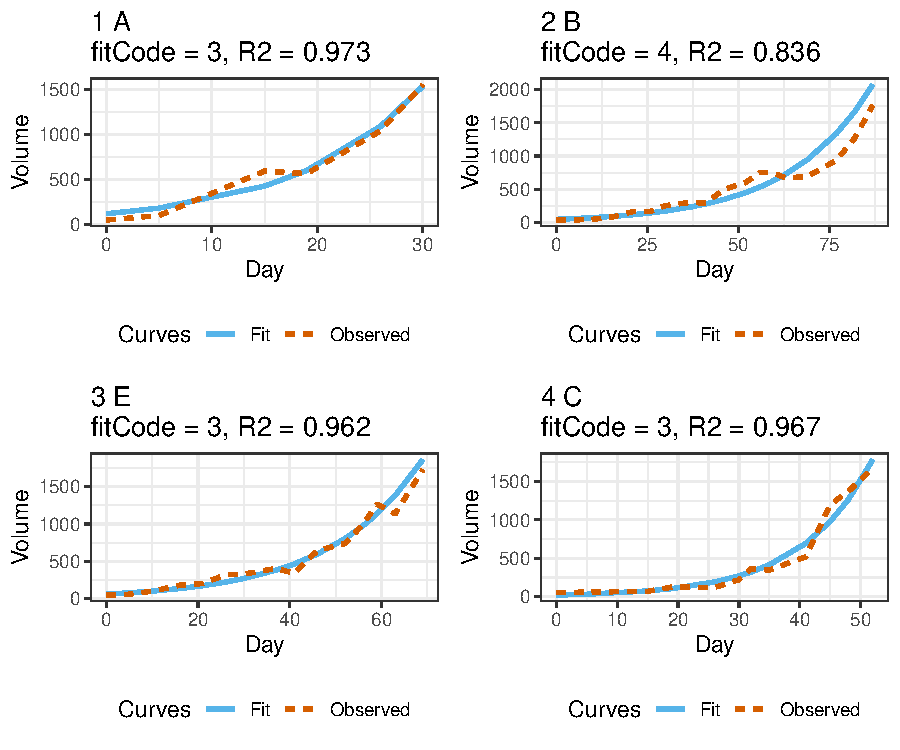
\includegraphics[width=0.9\textwidth]{img/mouse_fit.pdf}
\caption{Plot of \xt{mouse\_fit}, using \xt{data.table} syntax to subset to only the first four observations}
\label{fig:plot_fits}
\end{figure}

\subsection{Bootstrapping}

Once fits have been made, we are ready to begin estimating the group distributions and investigating temporal differences. This is done with the bootstrapping (and now permutation) function, \xt{bboot}. The number of options included in the \xt{bboot} function have expanded to include a new formula syntax for specifying the analysis of interest as well as to include options for permutation testing. A call to \xt{bboot} takes the following form

\begin{singlespace}
\begin{figure}[H]
\centering
\begin{BVerbatim}
bboot(formula, bdObj, B, alpha, permutation = TRUE, padj = "oleson", ...)
\end{BVerbatim}

\end{figure}
\end{singlespace}

The \xt{formula} argument is new to  \xt{bdots} and will be discussed in the next section. As for the remaining arguments, \xt{bdObj} is simply the object returned from \xt{bfit} that we wish to investigate, and \xt{B} serves the dual role of indicating the number of bootstraps/permutations we wish to perform. \xt{alpha} is the rate at which we wish to control the FWER. \xt{permutation} and \xt{padj} work in contrast to one another: when \xt{permutation = TRUE} (the default?), the argument to \xt{padj} is ignored. Otherwise, \xt{padj} indicates the method to be used in adjusting the nominal \xt{alpha} to control the FWER. By default, \xt{padj = "oleson"}. Finally, as previously mentioned, there is no longer a need to specify if the groups are paired, and \xt{bboot} determines this automatically based on the subject identifiers in each of the groups.


\paragraph{Formula}

As the \xt{bfit} function is now able to create fits for an arbitrary number of groups at once, we rely on a formula syntax in \xt{bboot} to specify precisely which groups differences we wish to compare. Let \xt{y} designate the outcome variable indicated in the \xt{bfit} function and let \xt{group} be one of the group column names to which our functions were fit. Further, let \xt{val1} and \xt{val2} be two values within the \xt{group} column. The general syntax for the \xt{bboot} function takes the following form:

\begin{singlespace}
\begin{figure}[H]
\centering
\begin{BVerbatim}
y ~ group(val1, val2)
\end{BVerbatim}
%\caption{Illustration of Mouse data}
\end{figure}
\end{singlespace}

Note that this is an \textit{expression} in R and is written without quotation marks. To give a more concrete example, suppose we wished to compare the difference in tumor growth curves for A and B from the \xt{Treatment} column in our mouse data (Figure~\ref{fig:mouse_head}). We would do so with the following syntax:

\begin{singlespace}
\begin{figure}[H]
\centering
\begin{BVerbatim}
Volume ~ Treatment(A, B)
\end{BVerbatim}
%\caption{Illustration of Mouse data}
\end{figure}
\end{singlespace}

There are two special cases to consider when writing this syntax. The first is the situation that arises in the case of multiple or nested groups, the second when a difference of difference analysis is conducted. Details on both of these cases are handled in the appendix. 



\paragraph{Summary and Analysis}

[what gets a paragraph, what gets a subsubsection?  compare this with \textit{\textbf{subsection}} for fitting]

Let's begin first by running \xt{bboot} using bootstrapping to compare the difference in tumor growth between treatment groups A and E in our mouse data using permutations to test for regions of significant difference. 

\begin{singlespace}
\begin{figure}[H]
\centering
\begin{BVerbatim}
mouse_boot <- bboot(Volume ~ Treatment(A, E), bdObj = mouse_fit, permutation = TRUE)
\end{BVerbatim}
%\caption{Illustration of Mouse data}
\end{figure}
\end{singlespace}


This returns an object of class \xt{bdotsBootObj}. A summary method is included to display relevant information:

\begin{singlespace}
\begin{figure}[H]
\centering
\begin{BVerbatim}
> summary(mouse_boot)

bdotsBoot Summary

Curve Type: expCurve 
Formula: Volume ~ x0 * exp(Day * k) 
Time Range: (0, 59) [21 points]

Difference of difference: FALSE 
Paired t-test: FALSE 
Difference: Treatment 

FWER adjust method: Permutation 
Alpha: 0.05 
Significant Intervals:
     [,1] [,2]
[1,]   15   32
\end{BVerbatim}
%\caption{Illustration of Mouse data}
\end{figure}
\end{singlespace}

There are a few components of the summary that are worth identifying when reporting the results. In particular, note the time range provided, an indicator of if the test was paired, and which groups were being considered \cn{(noticing now it only has \xt{Treatment}, not \xt{A} or \xt{E})}. The last section of the summary indicates the testing method used, an adjusted \xt{alphastar} if \xt{permutation = FALSE}, and a matrix of regions identified as being significantly different. This matrix is \xt{NULL} is no differences were identified at the specified alpha; otherwise there is one row included for each disjointed region of significant difference.

In addition to the provided summary output, a \xt{plot} method is available, with a list of additional options included in \xt{help(plot.bdotsBootObj)}.

\begin{figure}[H]
\centering
\begin{BVerbatim}
plot(mouse_boot)
\end{BVerbatim}

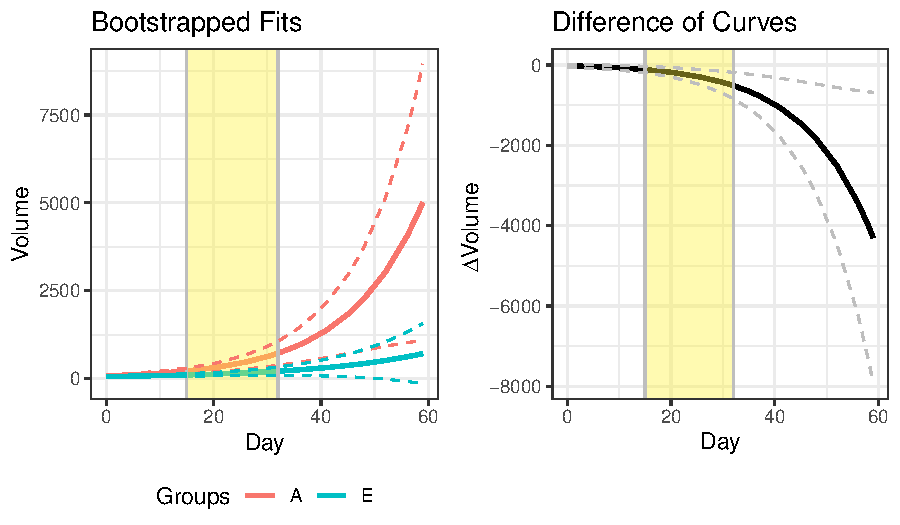
\includegraphics{img/mouse_boot_plot.pdf}
\caption{Bootstrapped distributions with regions of significant difference determined via permutation testing \cn{There are some obvious issues with time for non-homogenous samples, namely, what do we use for bootstrapping? It will be quick fix, whatever we decide, but I don't think ``union of all observed times" is going to work. Here, I artificially cut it back to only 0-60}}
\end{figure}
%
%Depending on user needs, these plots can be recreated both without confidence bands or without the additional difference curve
%
%\begin{figure}[H]
%\centering
%\begin{BVerbatim}
%plot(mouse_boot, ciBands = FALSE, plotDiffs = FALSE)
%
%\end{BVerbatim}
%
%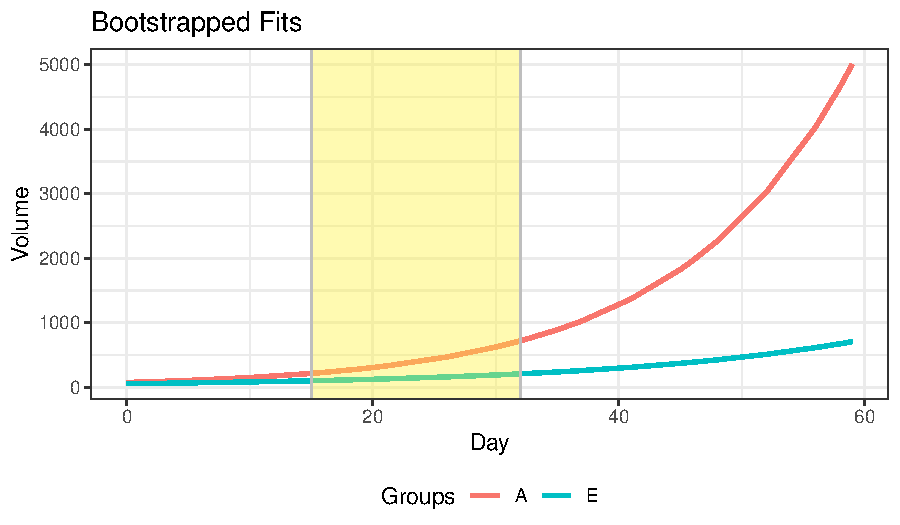
\includegraphics{img/mouse_boot_plot_extra.pdf}
%\caption{I think I'm going to actually not include this}
%\end{figure}


\section{Ancillary Functions}

Include here are a number of different function in \xt{bdots} facilitating  analysis but are otherwise not strictly necessary

\subsection{Refitting}

There are sometimes situations in which the fitted function returned by \texttt{bfit} is a poor fit. The nonlinear curve fitting algorithm used by \xt{nlme::gnls} in \xt{bfit} can be sensitive to starting parameters. Sensible starting parameters are computed from the observed data as part of the curve fitting functions (i.e., within the \xt{logistic()} function), though these can often be improved upon.


The quality of the fit can be evidenced by the \texttt{fitCode} or via a visual inspection of the fitted functions against the observations for each subject.  When this occurs, there are several options available to the user, all of which are provided through the function \texttt{brefit} (previously \texttt{bdotsRefit}). \texttt{brefit} takes the following arguments:

\begin{singlespace}
\begin{figure}[H]
\centering
\begin{BVerbatim}
brefit(bdObj, fitCode = 1L, subset = NULL, quickRefit = FALSE, paramDT = NULL)
\end{BVerbatim}
%\caption{Illustration of Mouse data}
\end{figure}
\end{singlespace}

The first of these arguments outside of the \xt{bdObj} is \xt{fitCode}, indicating the minimum fit code to be included in the refitting process. As discussed in Section~\ref{sec:fitcode}, this can be sub-optimal. To add flexibility to which subjects are fit there is now the \xt{subset} argument taking either a logical expression or collection of indices that would be used to subset an object of class \xt{data.table} (am I explaining this clearly?) or a numeric vector with indices that the user wishes to refit.

To assist with the refitting process is the argument \xt{quickRefit}. When set to \xt{TRUE}, \xt{brefit} will take the average coefficients of accepted fits within a group and use those as new starting parameters for poor fits. The new fits will be retained if they have a larger $R^2$ value by default. When set to \xt{quickRefit = FALSE}, the user will be guided through a set of prompts to refit each of the curves manually. 

Finally, the \texttt{paramDT} argument allows for a \xt{data.table} with columns for subject, group identifiers, and parameters to be passed in as a new set of starting parameters. This \xt{data.table} requires the same format as that returned by \xt{bdots::coefWriteout}. The use of this functionality is covered in more detail in the \xt{bdots} vignettes and is a useful way for reproducing a \xt{bdotsObj} from a plain text file. 

When \texttt{quickRefit = FALSE}, the user is put through a series of prompts along with a series of diagnostics for each of the subjects to be refit. Here, for example, is the option to refit subject 11 from the mouse data:


\begin{singlespace}
\begin{figure}[H]
\centering
\begin{BVerbatim}
Subject: 11
R2: 0.837
AR1: FALSE
rho: 0.9
fitCode: 4

 Model Parameters:
       x0         k 
53.186497  0.051749 

Actions:
1) Keep original fit
2) Jitter parameters
3) Adjust starting parameters manually
4) Remove AR1 assumption
5) See original fit metrics
6) Delete subject
99) Save and exit refitter
Choose (1-6):
\end{BVerbatim}
%\caption{Illustration of Mouse data}
\end{figure}
\end{singlespace}

There are a number of options provided in this list. The first, of course, keeps the original fit of the presented subject and moves on to the next subject in the list. The second option takes the values of the fitted parameter and ``jitters" them, changing each of the values by a prespecified magnitude. Given the sensitivity of \xt{nlme::gnls} to starting parameters, this is sometimes enough for the fitter to converge on a better fit for the observed data. Alternatively, the third option gives the user the ability to select the starting parameters manually. The third option gives the user the ability to attempting refitting the observed data without an AR(1) error assumption, though this is only relevant if such an assumption exists. Option (5) reprints summary information and the final option allows the user to delete the subject all together.

When any attempt to refit the observed under new conditions is presented (options (2)-(4)), a plot is rendered comparing the original fit side-by-side with the new alternative, Figure~\ref{fig:refit_plot}.

\begin{figure}[H]
\centering
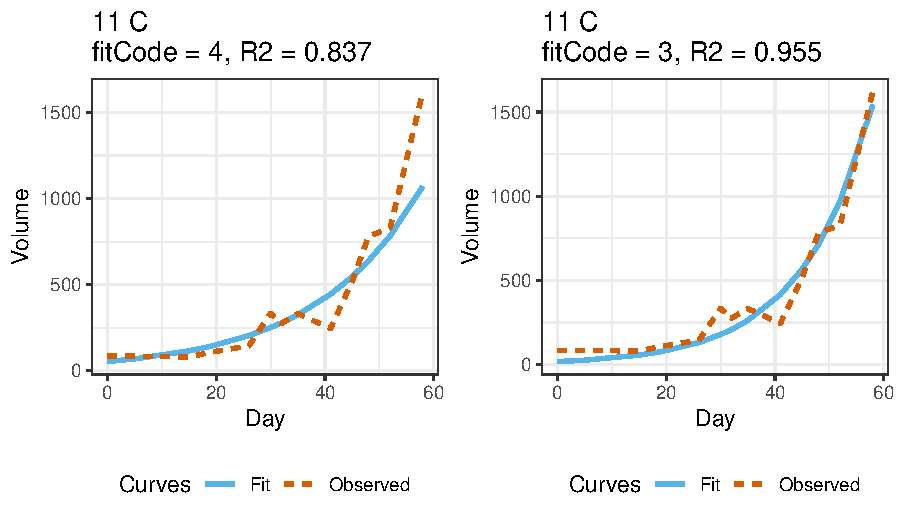
\includegraphics{img/mouse_refit_plot.pdf}
% new pars x0=50, k = 0.06
\caption{before and after refit}
\label{fig:refit_plot}
\end{figure}

As the menu item suggests, users have the ability to end the manually refitting process early and save where they had left off. To retain previously refit items and start again at a later time, pass the first refitted object back into the refitter as such:

\begin{singlespace}
\begin{figure}[H]
\centering
\begin{BVerbatim}
refit <- brefit(fit, ...)
refit <- brefit(refit, ...) # pass in the refitted object
\end{BVerbatim}
%\caption{Illustration of Mouse data}
\end{figure}
\end{singlespace}



A final note should be said regarding the option to delete a subject. As \xt{bdots} now automatically determines if subjects are paired based on subject identifiers (necessary for  calculations in significance testing), it is critical that if a subject has a poor fit in one group and must be removed that he or she is also removed from all additional groups in order to retain paired status. This can be overwritten with a final prompt in the \texttt{brefit} function before they are removed. The removal of subjects can also be done with the ancillary function, \texttt{bdRemove}, useful for removing subjects without undergoing the entire refitting process. See \xt{help(bdRemove)} for details.


\subsection{Correlations}

There are sometimes cases in which we are interested in determining the correlation of a fixed attribute with group outcome responses across time . This can be done with the \texttt{bcorr} function (previously \texttt{bdotsCorr}), which takes as an argument an object of class \texttt{bdotsObj} as well as a character vector representing a column from the original dataset used in \texttt{bfit}

\begin{center}
\xt{bcorr(fit, "value", ciBands, method = "pearson")} 
\end{center}

Need to elaborate here with example

\subsection{$\alpha$ Adjustment}

There may also be situations in which users wish to make an adjustment to autorcorrelated test statistics using the modified Bonferonni adjustment provided in \cite{oleson2017detecting}, though in a different context than what is done in \xt{bdots}. To facilitate this, we introduce an extension to the \texttt{p.adjust} function, \texttt{p\_adjust}, identical to \texttt{p.adjust} except that it accepts method \texttt{"oleson"} and takes additional arguments \texttt{rho}, and \texttt{df}. \texttt{rho} determines the autocorrelation estimate for the oleson adjustment while \texttt{df} returns the degrees of freedom used to compute the original vector of t-statistics. If an estimate of \texttt{rho} isn't available, one can be computed on a vector of t-statistics using the \texttt{ar1Solver} function in \xt{bdots}:

%\begin{center}
%\texttt{t <- diffinv(rnorm(100))} \\
%\texttt{rho <- ar1Solver(t)} \\
%\texttt{unadj\_p <- pt(t, df = 10)} \\
%\texttt{adj\_p <- p\_adjust(unadj\_p, method = "oleson", df = 10, rho = rho, alpha = 0.05)}
%\end{center}


\begin{singlespace}
\begin{figure}[H]
\centering
\begin{BVerbatim}
t       <- diffinv(rnorm(5))
rho     <- ar1Solver(t)
unadj_p <- pt(t, df = 10)
adj_p   <- p_adjust(unadj_p, method = "oleson", 
                    df = 10, rho = rho, alpha = 0.05)
\end{BVerbatim}
%\caption{Illustration of Mouse data}
\end{figure}
\end{singlespace}

The \xt{p\_adjust} function returns both adjusted p-values, which can be compared against the specified alpha (in this case, $0.05$) along with an estimate of alphastar, a nominal alpha at which one can compare the original p-values:

\begin{singlespace}
\begin{figure}[H]
\centering
\begin{BVerbatim}
> unadjp
[1] 0.5000000 0.0849965 0.0381715 0.1601033 0.0247453 0.0013016
> adjp
[1] 0.9201915 0.1564261 0.0702501 0.2946514 0.0455408 0.0023954
attr(,"alphastar")
[1] 0.027168
\end{BVerbatim}
%\caption{Illustration of Mouse data}
\end{figure}
\end{singlespace}

Here, for example, we see that the last two positions of \xt{unadjp} have values less than \xt{alphastar}, identifying them as significant; alternatively, we see these same two indices in \xt{adjp} significant when compared to \xt{alpha = 0.05}

\section{Discussion}


The original implementation of \xt{bdots} set out to address a narrow set of problems. Previous solutions beget new opportunities, however, and it is in this space that the second iteration of \xt{bdots} has sought to expand. Since then, the interface between user and application has been significantly revamped, creating a intuitive, reproducible workflow that is able to quickly and simply address a broader range of problems. The underlying methodology has also been improved and expanded upon, offering better control of the family-wise error rate.

While significant improvements have been made, there is room for further expansion. The most obvious of these is the need to include support for non-parametric functions, the utility of which cannot be overstated. Not only would this alleviate the need for the researcher to specify in advance a functional form for the data, it would implicitly accommodate more heterogeneity of functional forms within a group. Along with this, the current implementation is also limited in the quality-of-fit statistics used in the fitting steps to assess performance. $R^2$ and the presence of autocorrelation are relevant to only a subset of the types of data that can be fit, and allowing users more flexibility in specifying this metric is an active goal for future work. In all, future directions of this package will be primarily focused on user interface, non-parametric functions, and greater flexibility in defining metrics for fitted objects.



\section*{Appendix}

This section currently commented out. Involves instructions for fitting difference of difference and nested groups. Also may possibly include custom curve fitting.

%
%
%
%\section*{Appendix X} \\
%
%We will illustrate use of the updated \xt{bdots} package with a worked example, using an artificial dataset to help detail some of the newer aspects of the package. The dataset will consist of outcomes for a collection of vehicles, consisting of eight distinct groups. These groups will be nested in order of vehicle origin (foreign or domesetic), vehicle class (car or truck), and vehicle color (red or blue). Further, vehicles of different color but within the same origin and class groups will be considered paired observations. A table detailing the relationship of the groups is shown here:
%
%
%
%The outcome here is simply \xt{y} due to a lack of creativity, but the functional form assumed (and used in data generation) follows the four parameter logistic, 
%
%\begin{equation}
%f_{\theta}(t) = b + \frac{p-b}{1 + \exp \left( \frac{4s}{p-b} (x-t) \right)},
%\end{equation}
%where $b$, $p$, $s$, and $x$ represent the baseline, peak, slope, and crossover points, respectively
%
%
%
%The formula argument serves two functions in \xt{bboot}: first, it specifies the collection of curves we wish to investigate the difference between, and second, it determines if we are interested in directly comparing the differences or the difference of differences between curves. 
%
%To begin, let's reintroduce the structure of the groups we have in our dataset. Recall that we have foreign and domestic cars and trucks, and each of these vehicles comes in red and blue. Recall also that the different colors of each vehicle are considered paired observations.
%
%\begin{table}
%\centering
%\def\arraystretch{1.5}
%\begin{tabular}{|p{0.9in}|p{0.9in}|p{0.9in}|} \hline 
%\rowcolor{lightgray} \multicolumn{1}{|c|}{Origin} & \multicolumn{1}{c|}{Class} & \multicolumn{1}{c|}{Color}\\
%\hline
%\multirow{4}{*}{foreign} & \multirow{2}{*}{car} & red \\
%\hhline{~~-}
%& & blue \\
%\hhline{~--}
%& \multirow{2}{*}{truck} & red \\
%\hhline{~~-}
%& & blue \\
%\hline
%\multirow{4}{*}{domestic} & \multirow{2}{*}{car} & red \\
%\hhline{~~-}
%& & blue \\
%\hhline{~--}
%& \multirow{2}{*}{truck} & red \\
%\hhline{~~-}
%& & blue \\
%\hline
%\end{tabular}
%\caption{table of stuff}
%\label{tab:group_table}
%\end{table}
%
%
%Beginning with a simple case, suppose we want to investigate the difference in outcome between foreign and domestic vehicles. Notionally, we would write
%
%\begin{center}
%\tt y $\sim$ Origin(foreign, domestic).
%\end{center}
%
%
%Note that this involves the grouping variable, \xt{Origin}, with the two values we are interested in comparing, \xt{domestic} and \xt{foreign}. With this specification, the distribution of functions considered in \xt{domestic} include all red and blue domestic cars and trucks.
%
%
%If we wanted to limit our investigation to only foreign and domestic \textit{trucks}, we would do this by including an extra term specifying the group and the desired value. In this case, 
%
%\begin{center}
%\tt y $\sim$ Origin(foreign, domestic) + Class(truck).
%\end{center}
%To compare only foreign and domestic \textit{red} trucks, we would add an additional term for color:
%
%\begin{center}
%\tt y $\sim$ Origin(foreign, domestic) + Class(truck) + Color(red).
%\end{center}
%
%There are also instances in which we might be considered in the interaction of two groups. Although there is no native way to handle interactions in \xt{bdots}, this can be done indirectly through the difference of differences (McMurray et al 2019, though truthfully I still don't understand why). To illustrate, suppose we are interested in understanding how the color of the vehicle differentially impacts outcome based on the vehicle class. In such a case, we might look at the difference in outcome between red cars and red trucks, and then again the difference between blue cars and blue trucks. Any difference between these two differences would give information regarding the differential impact of color between each of the two classes. This is done in \xt{bdots} using the \xt{diffs} synatx in the formula:
%
%%\textbf{FOUND SOURCE FOR THIS:} \textit{McMurray, Klein-Packard, Tomblin 2019, real time mechanics..pg 7}
%
%\begin{center}
%\tt diffs(y, Class(car, truck)) $\sim$ Color(red, blue)
%\end{center}
%
%Here, the \textit{outcome} that we are considering is the difference between vehicle classes, with the outcome of interest being color. This is helpful in remembering which term goes on the LHS of the formula. 
%
%Similar as to the case before, if we wanted to limit this difference of differences investigation to only include domestic vehicles, we can do so by including an additional term:
%
%\begin{center}
%\tt diffs(y, Class(car, truck)) $\sim$ Color(red, blue) + Origin(domestic).
%\end{center}
%
%The formula syntax was originally contrived to make comparisons within groups or within nested groups. Conceivably, however, one could be interested in making the comparison between domestic red trucks and foreign blue cars. Doing so requires a bit of a work around. Examples detailing how one might go about doing this are included in appendix B. 
%
%\section*{Appendix B - Fitting non-nested groups}
%
%(currently just copy pasted from the body of document, not edited so no need to really review)
%
%First, there would be some function of sorts, something like \xt{makeUniqueGroups} which would create a new group column with each permutation of previous groups being given a unique identifier. Doing this on the vehicle example would look something like \xt{fit <- makeuniquewhatever} resulting in the following grouping structure (for example) (and maybe you could specify group name and values who knows, kinda like factor this is just a working thought example)
%
%\begin{center}
%
%\begin{tabular}{|p{0.9in}|p{0.9in}|p{0.9in}|p{0.5in}|} \hline 
%\rowcolor{lightgray} \multicolumn{1}{|c|}{Origin} & \multicolumn{1}{c|}{Class} & \multicolumn{1}{c|}{Color} & \multicolumn{1}{c|}{bgroup}\\
%\hline
%\multirow{4}{*}{foreign} & \multirow{2}{*}{car} & red & A\\
%\hhline{~~--}
%& & blue & B \\
%\hhline{~---}
%& \multirow{2}{*}{truck} & red & C\\
%\hhline{~~--}
%& & blue & D\\
%\hline
%\multirow{4}{*}{domestic} & \multirow{2}{*}{car} & red & E \\
%\hhline{~~--}
%& & blue & F\\
%\hhline{~---}
%& \multirow{2}{*}{truck} & red & G\\
%\hhline{~~--}
%& & blue & H\\
%\hline
%\end{tabular}
%\end{center}
%
%To then investigate differences in outcome between a foreign red car and a domestic blue truck would simply then be
%
%\begin{center}
%\tt y $\sim$ bgroup(A, H)
%\end{center}
%
%yeah not like sexy or anything but whatever it would work.
%
%
